\begin{figure}[ht]
 \centering
 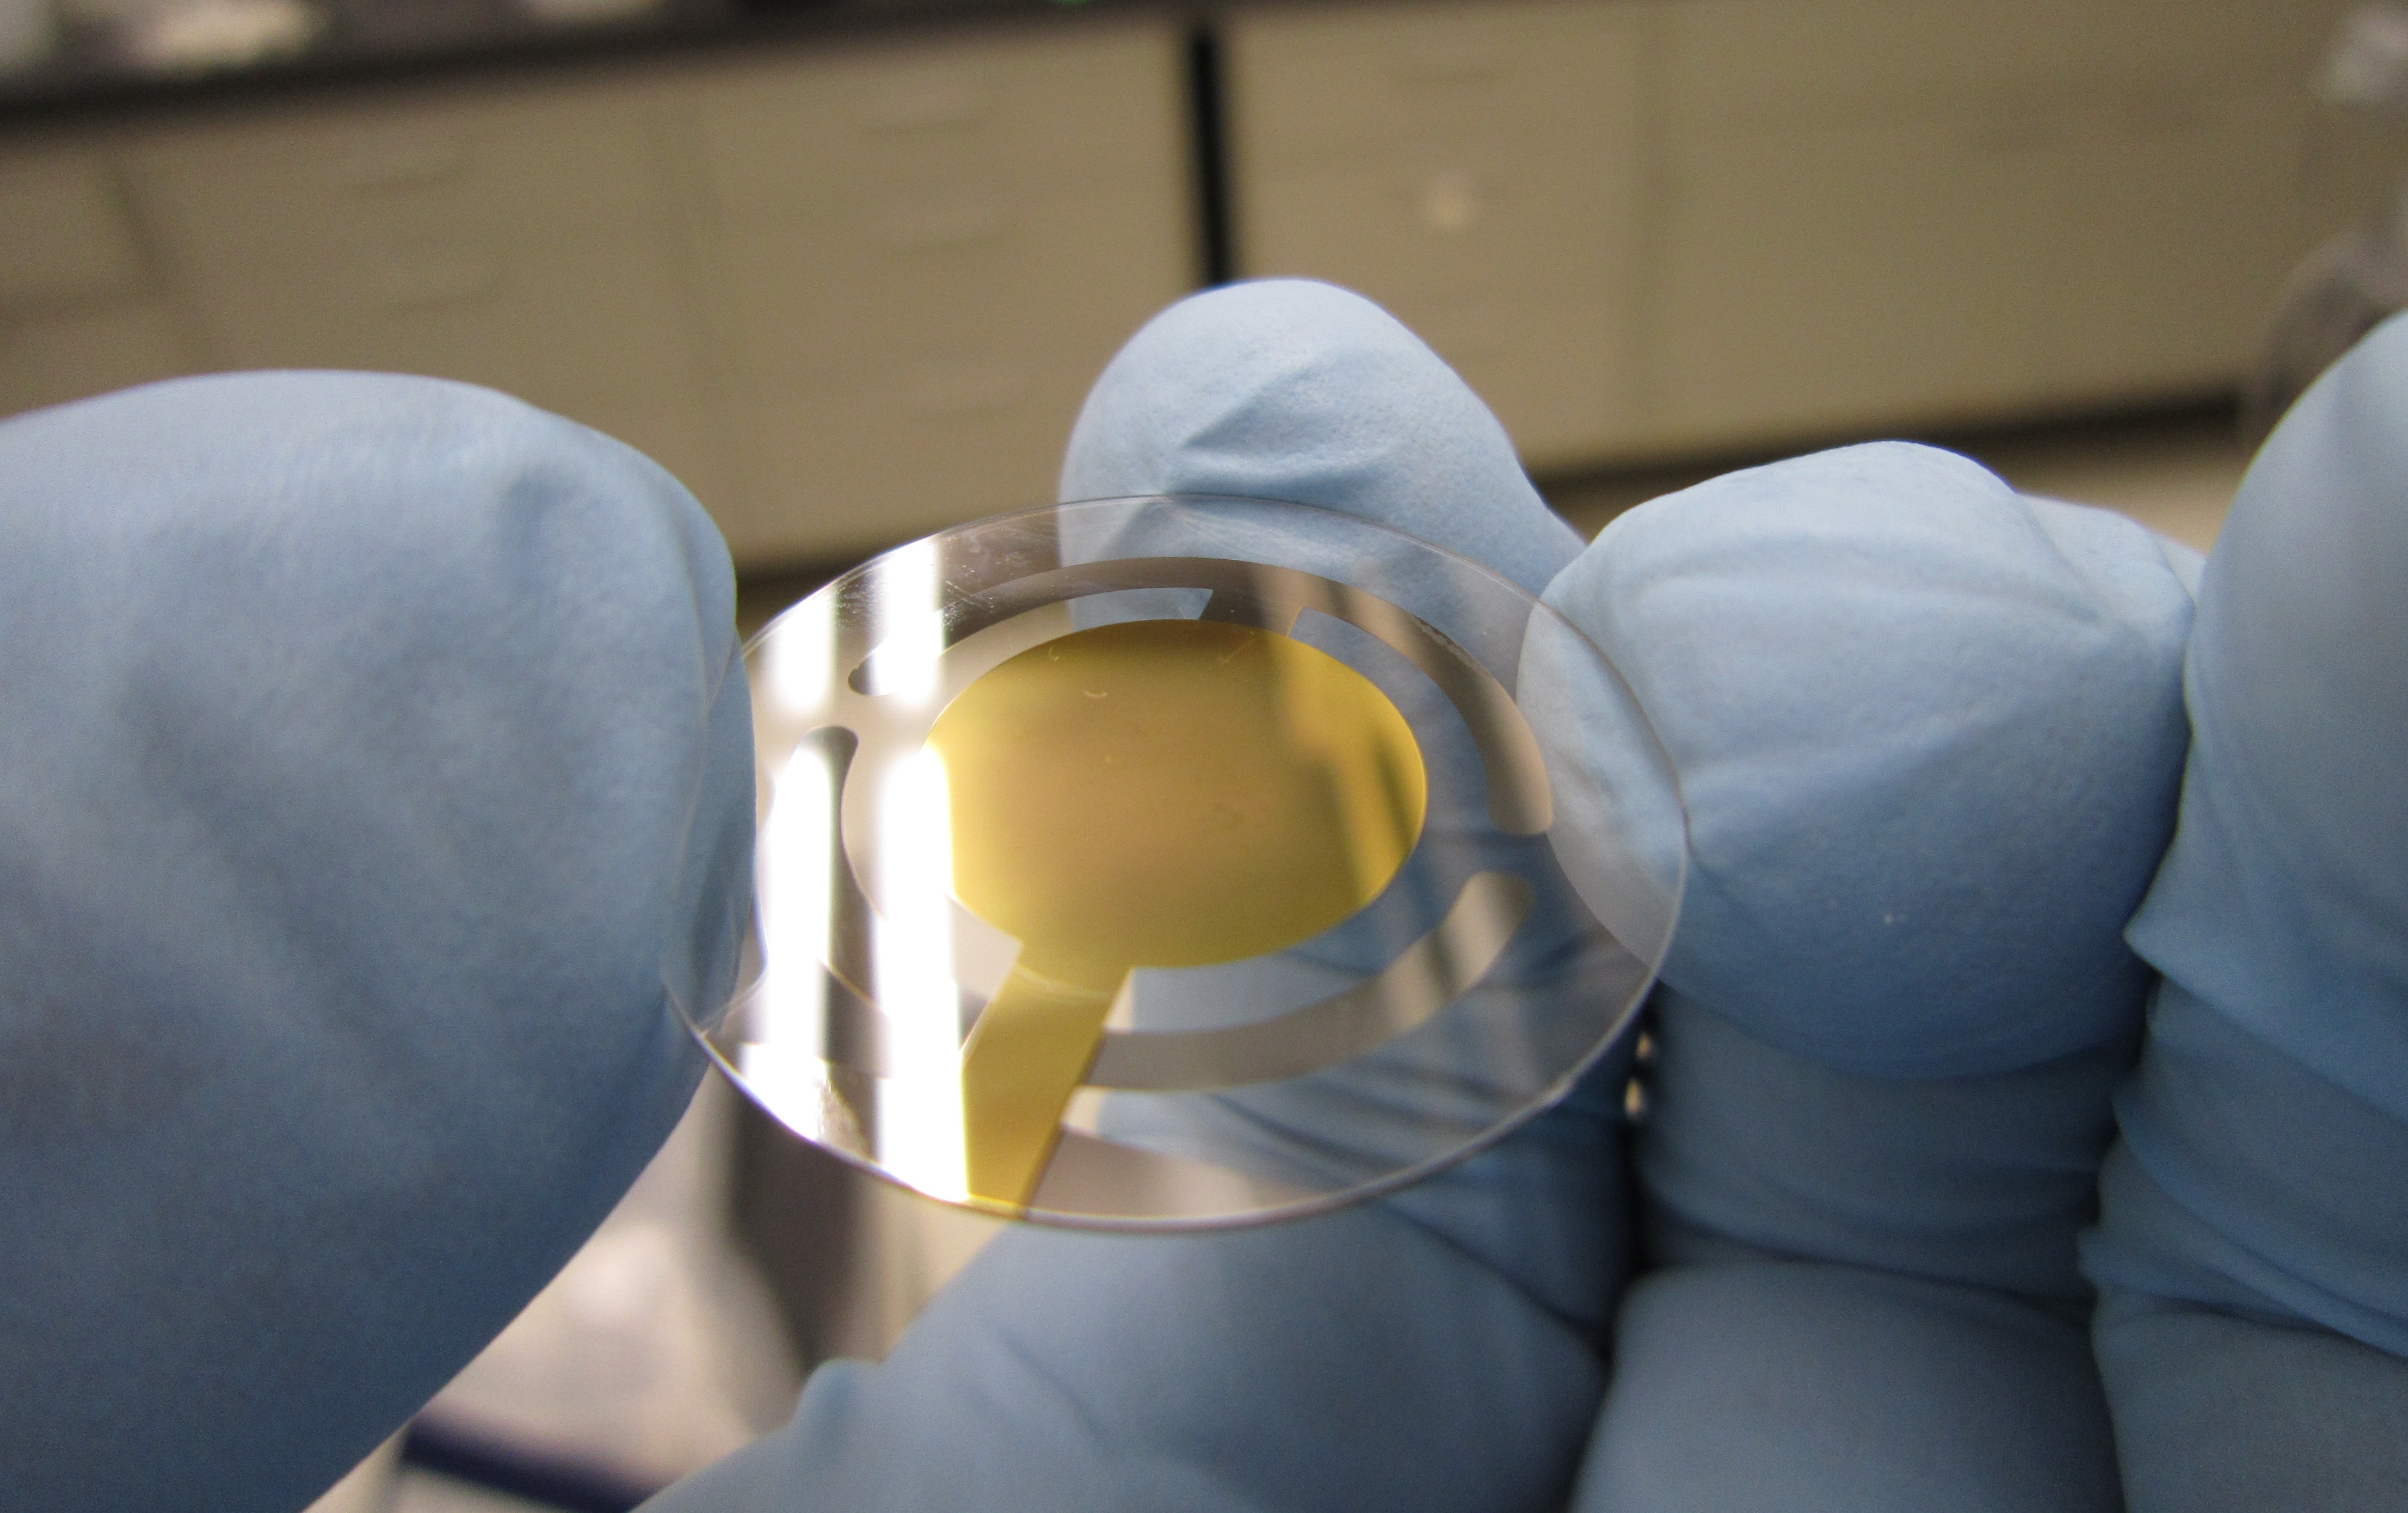
\includegraphics[keepaspectratio,width=10cm]{qcm/figures/qcm_holding.jpg}
 \caption{A quartz crystal microbalance in hand.}
 \label{fig:qcmholding}
\end{figure}

A quartz crystal microbalance is made of of a thin disc of crystalline
quartz, \ce{SiO2}, with metal electrodes deposited on either side
(\Figure{fig:qcmholding}).  The crystalline structure is specifically
$\alpha$-quartz, organized in a trigonal system which is pizeoelectric.
Typically the crystal employs the ``AT-cut'' -- a cut at an angle of
\SI{35.25}{\degree} with respect to the crystallographic axis.  In the
AT-cut, the vibrational state is dominated by the thickness shear mode,
setting up transverse shear waves along the faces of the crystal.  The
AT-cut quartz also has the desirable property of a zero frequency
temperature coefficent at \SI{25}{\celsius}.

\begin{figure}[ht]
 \centering
 %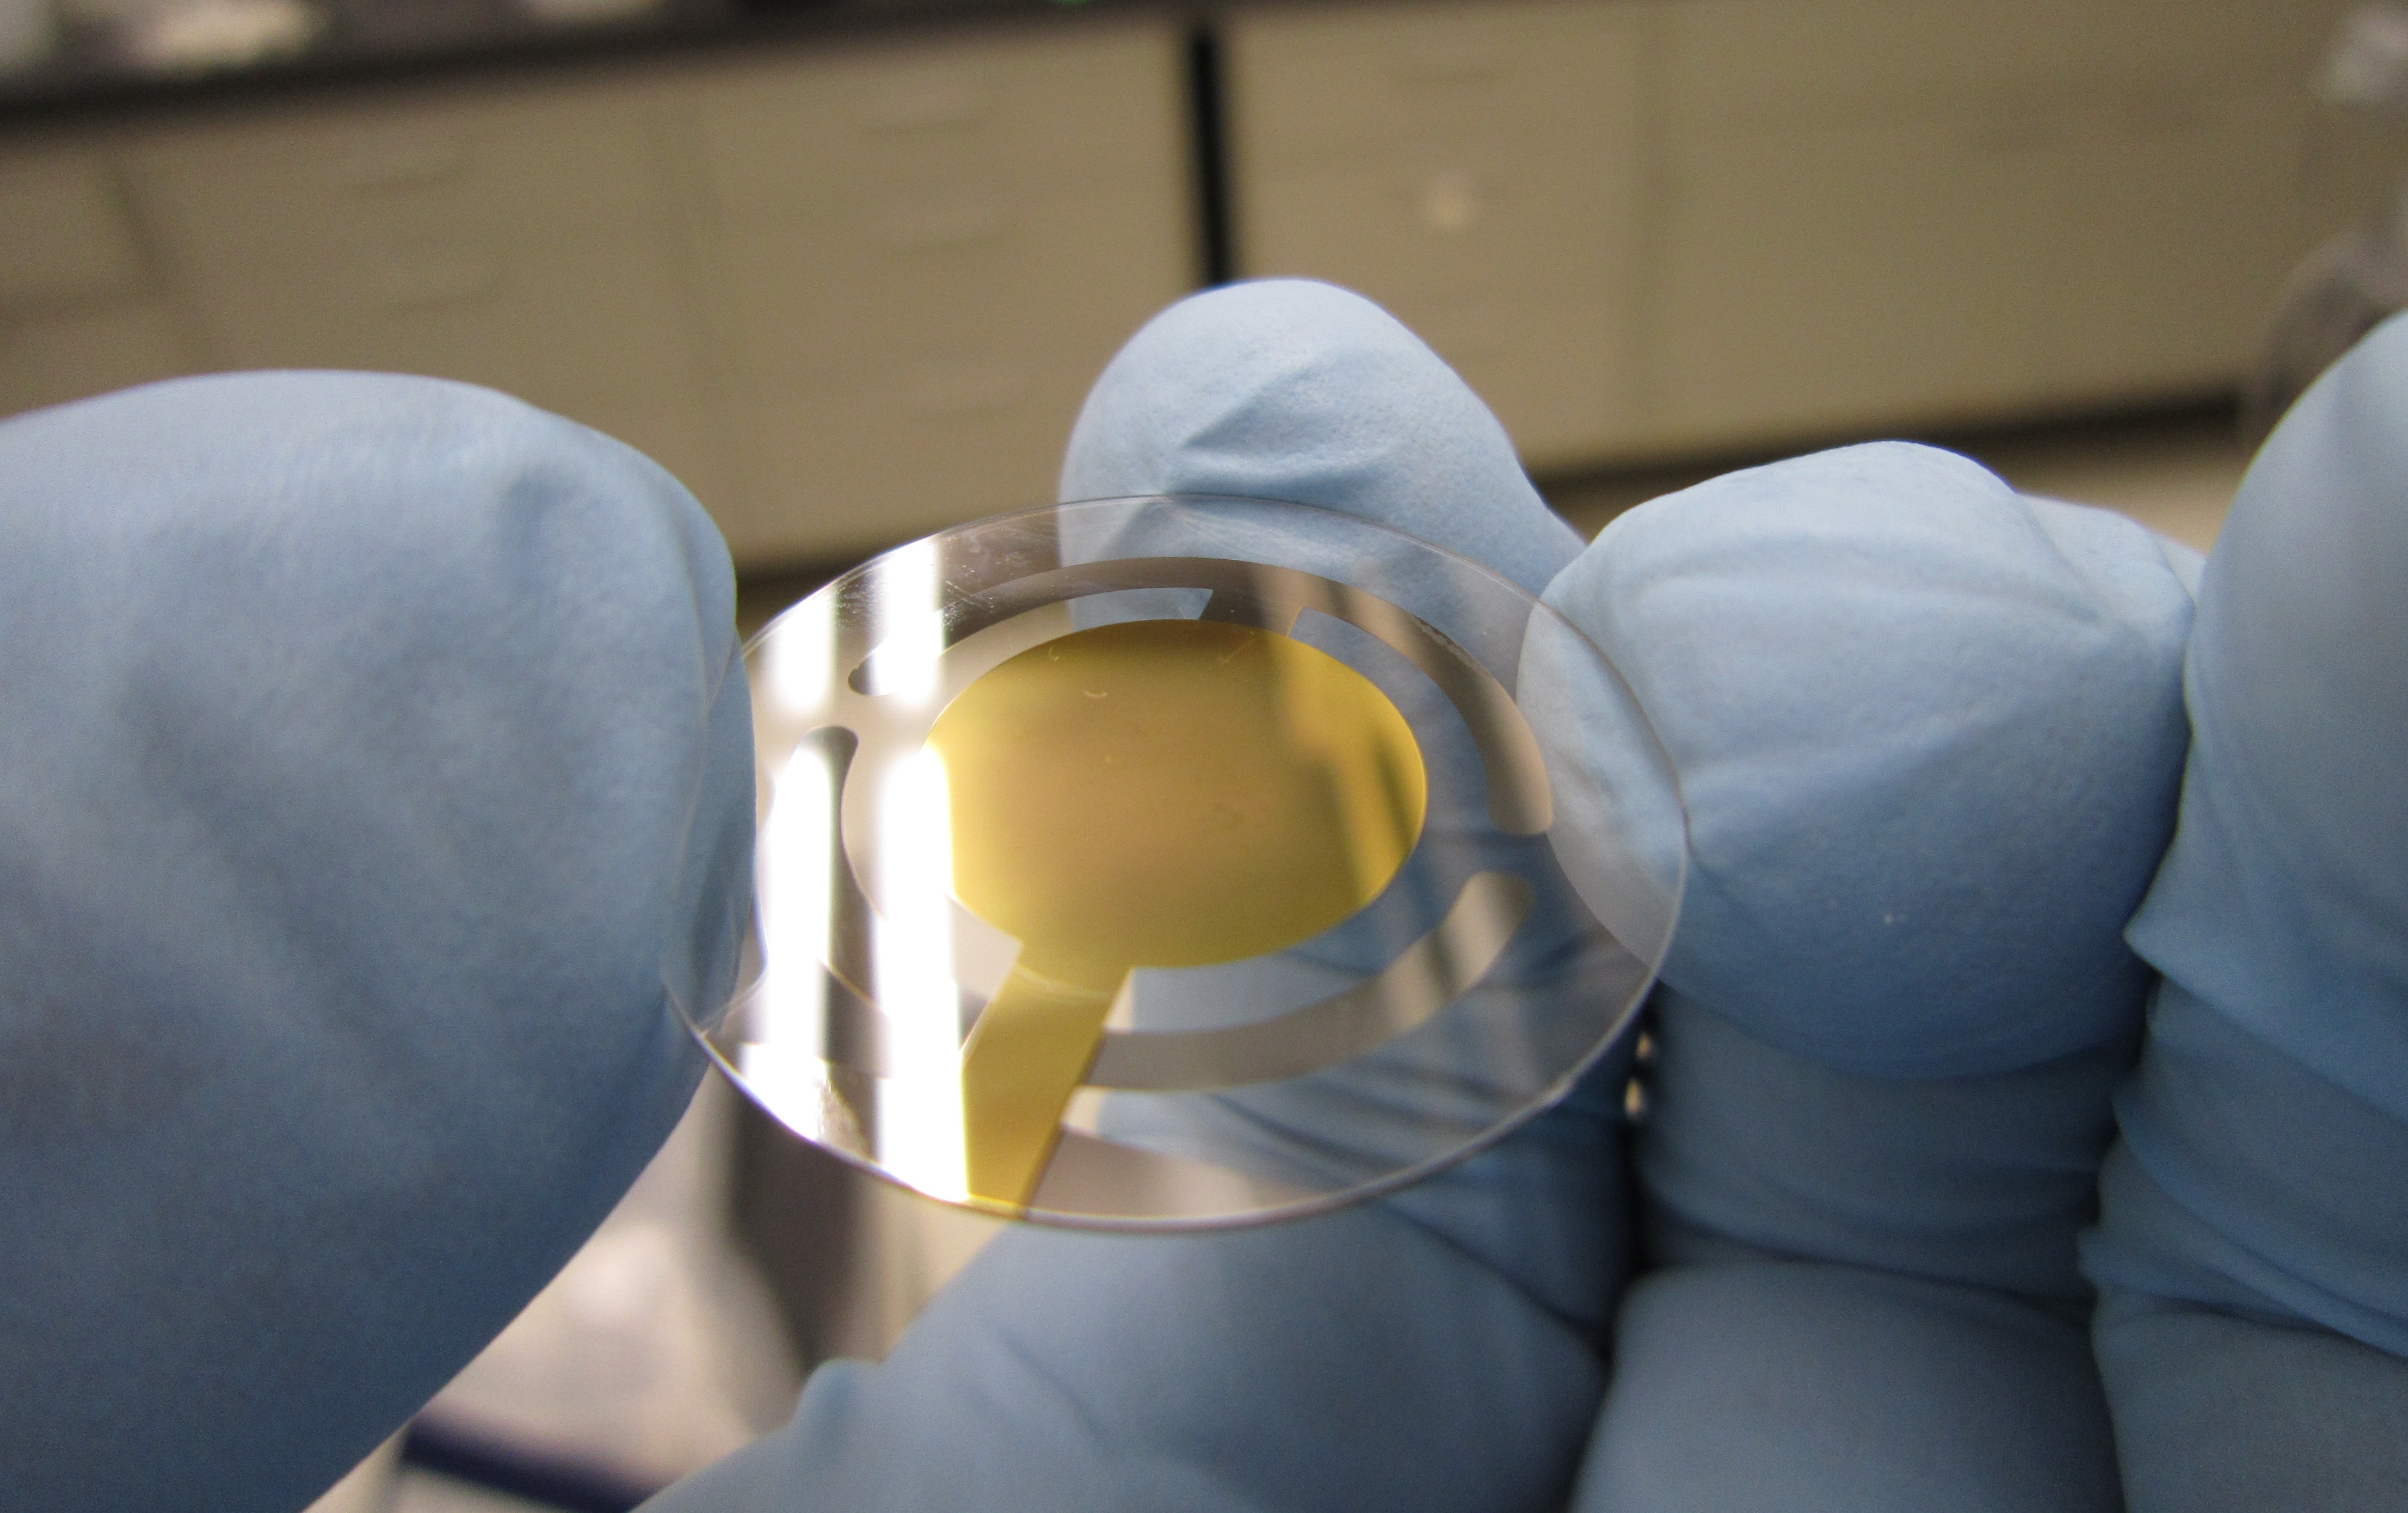
\includegraphics[keepaspectratio,width=10cm]{qcm/figures/qcm_holding.jpg}
	\caption{Conceptual drawing of a transverse shear wave.}
 \label{fig:qcmtsm}
\end{figure}

\subsection{Small Load Approximation}


Shifts in frequency, $\df$, and bandwidth (half-width at half maximum),
$\dg$, are computed by evaluating the stress-speed ratio of the oscillating
boundary according to the relationship
\begin{equation}
 \frac{\df+\mi\Delta\Gamma}{f_{\mathrm{F}}}=\frac{\mi}{\pi Z_{\mathrm{q}}}Z_\mathrm{L} =\frac{\mi}{\pi Z_{\mathrm{q}}}\left<\frac{\sigma}{\dot{u}}\right>
\label{eqn:comsolextract}
\end{equation}
where $\sigma$ is the (complex) stress, $\dot{u}$ is the (complex)
velocity, $Z_\mathrm{L}$ is the load impedance, and $\left<\enspace\right>$
denotes a line average along the boundary.  In \comsol, and in the
coordinates of \Figure{fig:compgeometry}, $\sigma$ is 
\texttt{Total stress, y component} (\texttt{v}) and $\dot{u}$ is 
\texttt{Velocity field, y component}, (\texttt{spf.T\_stressy}).  Note that
the stress speed ratio $\left<\sigma/\dot{u}\right>$ is dimensionally equivalent to
specific acoustic impedance, also called ``shock impedance'', sound
pressure over velocity.  In other words, the stress-speed ratio is the
impedance of the film. 

\begin{equation}
Z_\mathrm{L} = \left<\frac{\sigma}{\dot{u}}\right>
\label{eqn:comsolextract}
\end{equation}

%% small load approximation -> other paper -> equivalent mechanical model


As sensors, QCMs found their initial applications monitoring thin film
deposition in vacuums.  Here it was found that a QCM would exhibit a
frequency shift $\df$ proportional to the adsorbed mass $m$
\begin{equation}
 \df=-\frac{2f_{F}^{2}}{A\sqrt{\rho_{q}\mu_{q}}}\Delta m
 \label{eqn:sauerbrey}
\end{equation}
where $A$ is the active area of the crystal, $\Delta m$ is the adsorbed
mass, $\rho_{q}$ is the density of quartz and $\mu_{q}$ is the shear
modulus of quartz. Usually \Equation{eqn:sauerbrey} is condenced such that
$\Delta m$ is a linear function of a single ``sensitivity factor''
$C_\mathrm{f}$
\begin{equation}
 \Delta f=-C_{\text{f}}\Delta m
\end{equation}
where $C_{\text{f}}=\SI{56.6}{\hertz\per\micro\gram\centi\meter\squared}$.
\Equation{eqn:sauerbrey} is known as the
\textit{Sauerbrey relation}.  A typical QCM might have a
$f_F=\SI{5}{\mega\hertz}$ and a frequency resolution of \SI{0.1}{\hertz};
\Equation{eqn:sauerbrey} predicts sub-monolayer (and is only valid in this
range) resolution of the thickness
metal and dielectric layers.  This is the reason the name QCM includes the
word ``microbalance''.

Initially it was thought that the low $Q$ mechanical resonance of the QCM
precluded its use in the liquid phase.  This was incorrect, as subsequent
work published in 1985 by \name{Gordon} and \name{Kanazawa}~\cite{guys} extended the
treatment of \name{Sauerbrey} to the liquid phase.  These relations,
derived from a Butterworth van Dyke equivalent circuit, predicted the
resonant frequency of the QCM
to be sensitive to the density-viscosity product of the liquid in contact
with the crystal, 
\begin{align}
\df=&-f_{\text{F}}^{3/2}\left(\frac{\rho_{\text{L}}\eta_{\text{L}}}{\pi\rho_{q}\mu_{q}}\right)^{1/2}\\
\Delta R=&2f_{\text{F}}L\left(\frac{4\pi
 f_{\text{F}}\rho_{\text{L}}\eta_{\text{L}}}{\rho_{q}\mu_{q}}\right)^{1/2}
\end{align}
where $\rho_{\text{L}}$ and $\eta_{\text{L}}$ are the unknown density and
viscosity of the liquid.  Note that in the treatment by both Sauerbrey and
Gordon and Kanazawa, the frequency shifts are always \textit{negative} as a
function of increasing mass or density-viscosity.

The same year, \name{G. Dybwad} published a rather elegant
experiment~\cite{dybwad} in which he looked at the frequency shift of a QCM
in air when a single micron sized gold particle rests on the sensor
surface.  Remarkably, \name{Dybwad} reported a \textit{positive}
frequency shift.  The shift was explained with a coupled oscillator model
shown in \Figure{fig:dybwad}.
%\begin{figure}
% \caption{Coupled oscillator model used by \name{Dybwad}.}
% \label{fig:dybwadschema}
%\end{figure}
Here, the quartz crystal with mass $\mq$ and stiffness
$\kq$ resonates at
$\omega_\mathrm{q}^2=\kq/\mq$ and is coupled by a spring
$\kl$ to a load mass $\ml$.  The load mass is the actual mass of
the particle, $4/3 \pi r^3 \rho$.  The spring $\kl$ represents the
``stiffness'' of the contact -- how strongly the particle is coupled to the
QCM surface.  The coupled system in \Figure{fig:dybwadschema} is described
by the differential equations
\begin{align}
 \mq \ddot{x}_\mathrm{q} &= -\kq x_\mathrm{q}\\
 \ml \ddot{x}_\mathrm{L} &= -\kl (x_\mathrm{q}-x_\mathrm{L})
\end{align}
which, using an ansatz of
$x_{\mathrm{q},\mathrm{L}}=A_{\mathrm{q},\mathrm{L}}\me^{\mi \omega t}$ has
eigenvalues $\omega$ of
\begin{equation}
 2\omega^{2}=\left(\frac{\kq}{\mq}+\frac{\kl}{\mq}+\frac{\kl}{m}\right)\pm\left(\left(\frac{\kq}{\mq}+\frac{\kl}{\mq}+\frac{\kl}{\ml}\right)^{2}-4\frac{\kq}{\mq}\frac{\kl}{\ml}\right)^{1/2}
 \label{eqn:dybwadresult}
\end{equation}

%\begin{figure}
% \caption{Resonant frequency of the Dybwad model as a function of coupling
%  strength, $\kl$.}
% \label{fig:dybwadplot}
%\end{figure}
\Equation{eqn:dybwadresult}, shown in \Figure{fig:dybwadplot} has two
important limits about $\omegaq^2 \ml$
\begin{align}
 \lim_{\kl\to\infty} \omega^2 &= \frac{\kq}{\mq+\ml}\\
 \lim_{\kl\to0} \omega^2 &= \frac{\kq}{\mq}
\end{align}
In the weak coupling regime, $\kl\ll\omegaq^2\ml$, the particle causes a
positive frequency shift proportional to $\kl$ and independent of $\ml$.
Indeeed, in \name{Dybwad}'s model, in the weak coupling regime the
particle is seen to be at rest in the labratory frame. In the limit of strong
coupling, $\kl\gg\omegaq^2\ml$, the mass adsorption predicted by
\name{Sauerbrey} takes over.  Dybwad's work is important because it
establishes a continuum model for QCM behavior, encompassing both positive
and negative frequency shifts.

Some dingus guys use a nanoindenter probe combined with a QCM, this is
where we jump off.

Last, Yuki got the idea from other applicaions of force on stuff done by
Ken and Wesley.  So plan to jump into the main text.

